\documentclass[a4paper,11pt]{jsarticle}


% 数式
\usepackage{amsmath,amsfonts,amssymb}
\usepackage{bm}
% 画像
\usepackage[dvipdfmx]{graphicx}
\usepackage[dvipdfmx]{color}
\usepackage{siunitx}
\usepackage{wrapfig}
\usepackage{cases}
\usepackage{dcolumn}
\usepackage{subcaption}


% add hyperlinks
\usepackage[dvipdfmx]{hyperref}
\usepackage{pxjahyper}
\hypersetup{
  colorlinks=true,
  linkcolor=blue,
  citecolor=blue,
  breaklinks=true, 
}

% next page in align
\allowdisplaybreaks[1]

\begin{document}

\title{回転軸が円周上を自由に動く剛体単振り子について}
\author{Hiro Hirabayashi}
\date{\today}
\maketitle

\section{上肢と胴体が一致する角度が持つ力学的重要な意味について}

上肢が全身の質量に対して十分に軽いとし、
上肢の質量と慣性モーメントを$0$とするモデルを考える。
また、単純化のために股関節は真っすぐに完全に保たれるとする。
この時モデルは、
回転軸が円周上に自由に動く剛体単振り子になる。

\begin{figure}[h]
  \centering
  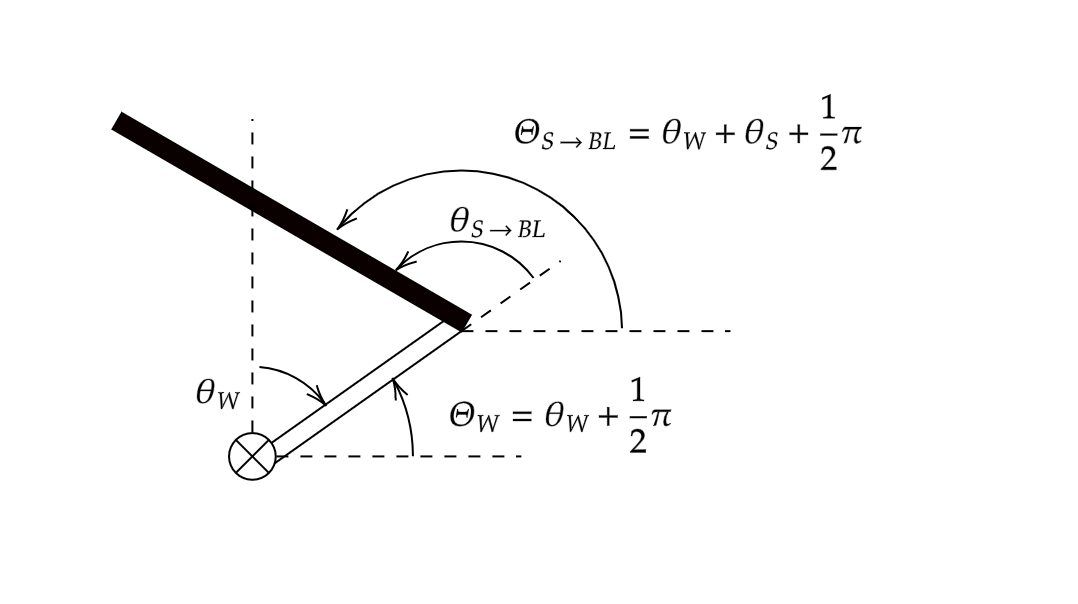
\includegraphics[width = 0.6\textwidth]{config.png}
  \caption{基本モデル}
  \label{config.png}
\end{figure}

\subsection{上肢の運動の決まり方}

上肢の慣性がなくなり、
0でない外力が働くと加速度が定義できなくなってしまうこのモデルに関して
運動方程式が成り立たないのではないか、
という疑問を持つだろう。
力学的な話をせずに、
このモデルに対してしっかりと運動方程式が成り立つことを説明するには、
上肢の存在を無視し、
肩関節に相当する部分が、円形のカーテンレールに固定されている状況を考えるとよい。
剛体単振り子の運動によって端点はカーテンレール上を摩擦なく動く。
このように考えれば、
現実に運動が成り立つことが想像できるだろう。

しかし、今回の議論では
上肢の慣性を無視したことや、
上肢の方向がとても大きな意味を持つ。
だから
0でない外力が働くと定義できなくなってしまう
上肢の加速度がどのように定まるのかを説明する。
ただし、簡単のため、手関節、肩関節にトルクを発生させない場合を考える。

\begin{figure}[h]
  \centering
  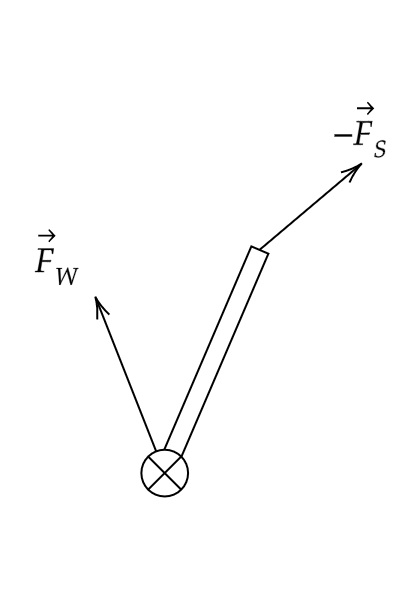
\includegraphics[width = 0.6\textwidth]{F_arm_config.png}
  \caption{上肢に働く力}
  \label{F_arm_config.png}
\end{figure}

上肢の手関節側(固定点)に働く力を$\vec{F}_W$、
肩関節側に働く力を$-\vec{F}_S$とする。
肩関節側に働く力は反作用として定義しておく。
上肢に関する並進運動のつり合いを考えると
\begin{align}
  0 \cdot \vec{a}_{Arm} &= \vec{F}_W - \vec{F}_S
  \\
  \Leftrightarrow
  0 &= \vec{F}_W - \vec{F}_S
\end{align}
が導かれるから、
$\vec{F}_W$と$-\vec{F}_S$は
方向が同じで、大きさが反対である力である。
また、手関節周りのトルクに関するつり合いを考えると
上肢の長さを$r_{Arm}$、
手関節から肩関節に向く方向単位ベクトルを$\vec{e}_{Arm}$とすれば
\begin{align}
  0 \cdot \omega_{Arm} &= r_{Arm} \vec{e}_{Arm} \times -\vec{F}_S
  \\
  \Leftrightarrow
  0 &= r_{Arm} \vec{e}_{Arm} \times -\vec{F}_S
  \\
  \Leftrightarrow
  \vec{e}_{Arm} &\parallel \vec{-F_S}
\end{align}
よって上肢の肩関節側に働く力$-\vec{F}_S$は
上肢と平行であり、
ゆえに上肢の手関節側に働く力$\vec{F}_W$も上肢と平行になる。
このことから、上肢には上肢と同じ方向に力がかかるが、
垂直な方向には力が加わらないことが分かる。
これではまだ上肢の加速度を決定することはできない。

そして次に考えるのが、
肩関節以降の剛体単振り子である。
セクション\ref{sec:appendix}に書いたが、
回転軸が固定される状況では
剛体単振り子が剛体単振り子であるには
向心力を必要とする。
しかし、絶対座標系から見ると
剛体の回転軸はそもそも固定されていない。
だから回転軸を固定した座標系をとる。
すなわち、肩関節に固定した座標系を考える。

\begin{figure}[h]
  \begin{tabular}{cc}
    \begin{minipage}[t]{0.45\textwidth}
      \centering
      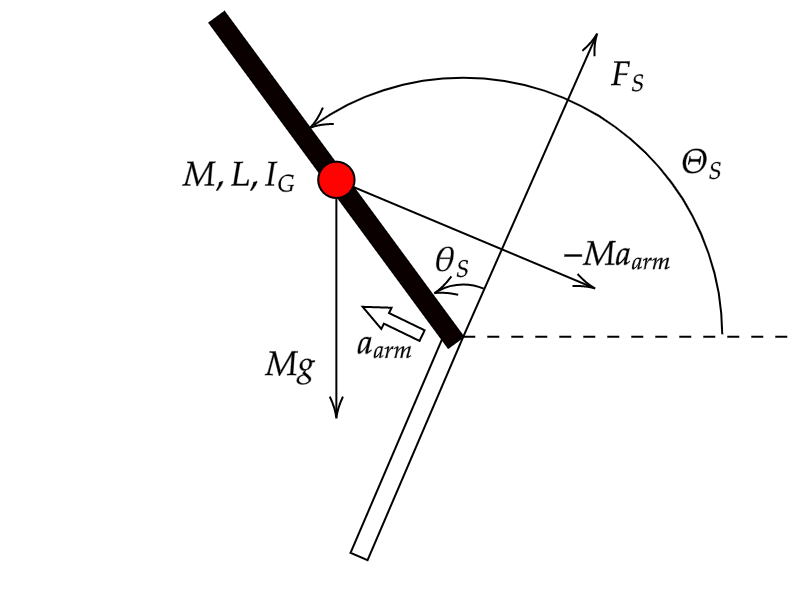
\includegraphics[width=1\textwidth]{1seg_F_config_for_FsMa.png}
      \subcaption{$F_S$と$Ma_{arm}$の係数について考えやすい状況}
      \label{1seg_F_config_for_FsMa.png}
    \end{minipage} &
    \begin{minipage}[t]{0.45\textwidth}
      \centering
      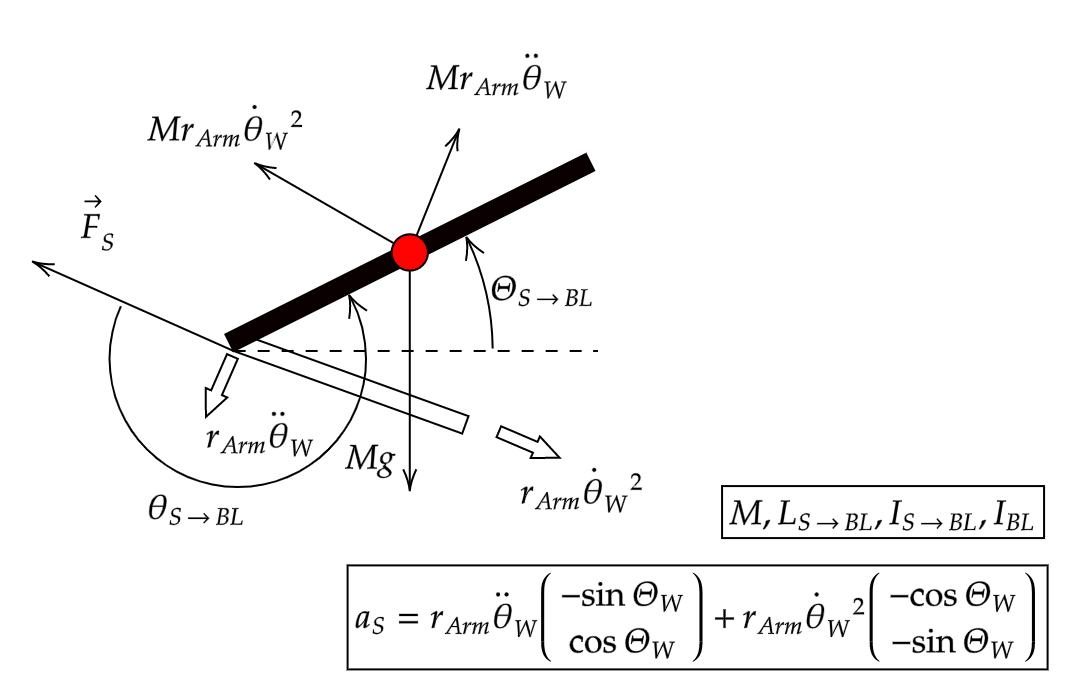
\includegraphics[width=1\textwidth]{1seg_F_config_for_Mg.png}
      \subcaption{重力$Mg$の係数について考えやすい状況}
      \label{1seg_F_config_for_Mg.png}
    \end{minipage}
  \end{tabular}
  \caption{剛体単振り子として見た場合の状況}
\end{figure}

肩関節の位置は等速度運動をしないから、
この座標上で物体の運動を考えるときは慣性力を考慮する必要があり、
運動方程式は
慣性力を$Ma_{arm}$として
\begin{align}
  ML\omega^2 &= Mg\sin\Theta_S &+& Ma_{arm}\sin\theta_S &- F_S\cos\theta_S
  \label{eq:PB:L_start}
  \\
  I\dot\omega &= -Mg\cos\Theta_S \cdot L &-& Ma_{arm}\cos\theta_S \cdot L &
  \label{eq:PB:I_start}
  \\
  I_G\dot\omega &= & & & F_S \sin\theta_S \cdot L
  \label{eq:PB:IG_start}
\end{align}
となる。
まず式\ref{eq:PB:I_start}, \ref{eq:PB:IG_start}によって
\begin{align}
  F_S\sin\theta_S \cdot L 
  & = I_G \cdot \frac{-Mg\cos\Theta_S \cdot L - Ma_{arm}\cos\theta_S \cdot L}{I}
  \\
  \left( \because L > 0 \right) &
  \\
  \Leftrightarrow
  F_S\sin\theta_S
  & = \frac{I_G}{I}\Bigl( -Mg\cos\Theta_S - Ma_{arm}\cos\theta_S \Bigr)
  \\
  \Leftrightarrow
  0
  & = F_S\sin\theta_S - \frac{I_G}{I}\Bigl( -Mg\cos\Theta_S - Ma_{arm}\cos\theta_S \Bigr)
  \\
  \Leftrightarrow
  0
  & = F_S\sin\theta_S + Mg\frac{I_G}{I}\cos\Theta_S + Ma_{arm}\frac{I_G}{I}\cos\theta_S
  \label{eq:PB:Fs_sin}
\end{align}
式\ref{eq:PB:L_start},\ref{eq:PB:Fs_sin}を変形して
\begin{align}
  ML\omega^2 \sin\theta_S &= Mg\sin\Theta_S \sin\theta_S
  &+& Ma_{arm}\sin^2\theta_S 
  &- F_S\cos\theta_S\sin\theta_S
  \\
  0
  &=  Mg\frac{I_G}{I}\cos\Theta_S\cos\theta_S 
  &+& Ma_{arm}\frac{I_G}{I}\cos^2\theta_S 
  &+ F_S\sin\theta_S\cos\theta_S
\end{align}
この2式から
\begin{align}
  ML\omega^2 \sin\theta_S
  = Mg\left( \sin\Theta_S \sin\theta_S + \frac{I_G}{I}\cos\Theta_S \cos\theta_S \right)
  + Ma_{arm}\left( \sin^2\theta_S + \frac{I_G}{I}\cos^2\theta_S \right)
\end{align}
\begin{align}
  \Leftrightarrow
  Ma_{arm}\left( \sin^2\theta_S + \frac{I_G}{I}\cos^2\theta_S \right)
  = ML\omega^2 \sin\theta_S
  - Mg\left( \sin\Theta_S \sin\theta_S + \frac{I_G}{I}\cos\Theta_S \cos\theta_S \right)
  \label{eq:PB:a_arm_end}
\end{align}
が分かる。
$\sin^2\theta_S + \frac{I_G}{I}\cos^2\theta_S > 0$であるから、
$a_{arm}$の符号は右辺で決まることになる。

\subsection{胴体と上肢の位置関係と上肢の加速方向}

上肢の加速を表す式\ref{eq:PB:a_arm_end}について
具体的な状況
\begin{enumerate}
  \item $\omega^2$が大きく、向心力ないし遠心力が十分に大きい場合
  \item $\omega^2$が小さく、向心力ないし遠心力が十分に小さい場合
  
  (しかしこちらのケースは時間が短く、影響力が大きくない。)
  *要データ確認(シミュレーション中の各項に相当するものの大きさ?)
\end{enumerate}
を考えることで理解を深めよう。


\begin{enumerate}
  \item $\omega^2$が大きく、向心力ないし遠心力が十分に大きい場合
  \begin{align}
    Ma_{arm}\left( \sin^2\theta_S + \frac{I_G}{I}\cos^2\theta_S \right)
    \approx ML\omega^2 \sin\theta_S
  \end{align}
  という近似が成り立つから、
  $\sin\theta_S$によって正負が決定される。
  上肢が正の方向に加速するのは
  $0<\theta_S<\pi$の時であり、
  つまり
  図\ref{PN_omega_positive.png}のような
  胴体が上肢より左側にある状況であり、
  上肢の角度や胴体の角度に依らない。
  逆に上肢が負の方向に加速するのは
  $\pi<\theta_S<2\pi$の時であり、
  つまり
  図\ref{PN_omega_negative.png}のような
  胴体が上肢より右側にある状況であり、
  上肢の角度や胴体の角度に依らない。
  これはまるで向心力ないし遠心力によって
  上肢が胴体のある方向に引っ張られていることを想起する。

  \begin{figure}[h]
    \begin{tabular}{cc}
      \begin{minipage}[t]{0.45\textwidth}
        \centering
        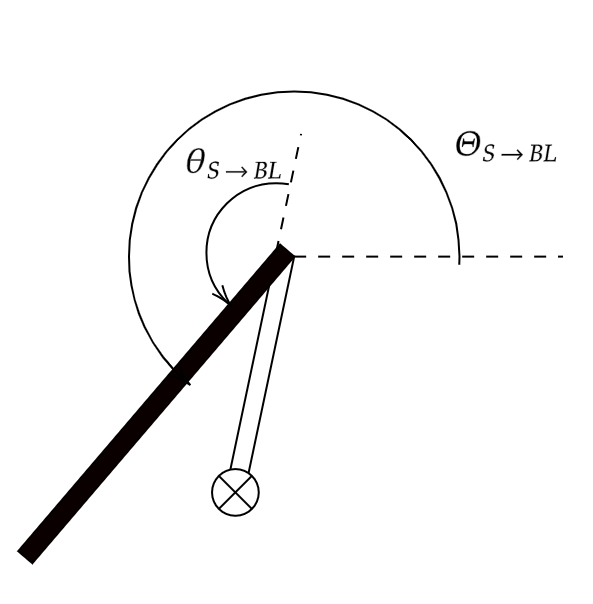
\includegraphics[width=1\textwidth]{PN_omega_positive.png}
        \subcaption{$a_{arm}$が正のケース}
        \label{PN_omega_positive.png}
      \end{minipage} &
      \begin{minipage}[t]{0.45\textwidth}
        \centering
        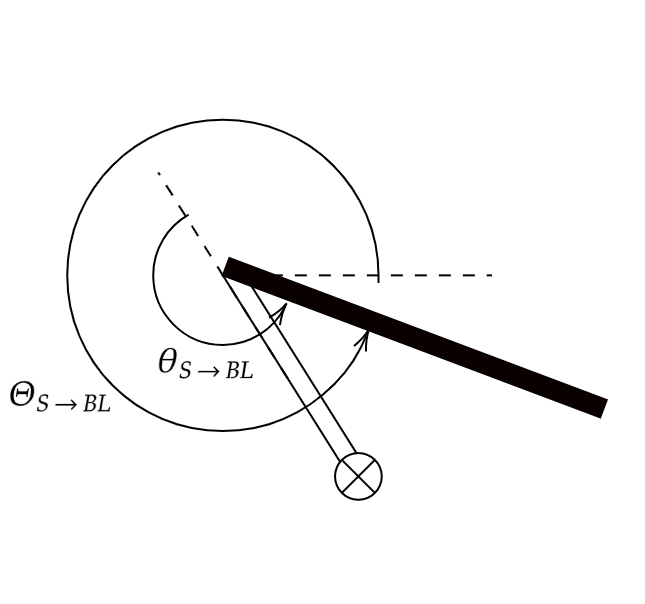
\includegraphics[width=1\textwidth]{PN_omega_negative.png}
        \subcaption{$a_{arm}$が負のケース}
        \label{PN_omega_negative.png}
      \end{minipage}
    \end{tabular}
    \caption{$\omega^2$が大きく、遠心力が大きいとき}
  \end{figure}

  \item $\omega^2$が小さく、向心力ないし遠心力が十分に小さい場合
  \begin{align}
    Ma_{arm}\left( \sin^2\theta_S + \frac{I_G}{I}\cos^2\theta_S \right)
    \approx - Mg\left( \sin\Theta_S \sin\theta_S + \frac{I_G}{I}\cos\Theta_S \cos\theta_S \right)  
  \end{align}
  という近似が成り立つから、
  $-\left(\sin\Theta_S \sin\theta_S + \frac{I_G}{I}\cos\Theta_S \cos\theta_S\right)$
  によって正負が決定する。
  例えば$\Theta_S = \pi$である状況では
  \begin{align}
    -\left(\sin\Theta_S \sin\theta_S + \frac{I_G}{I}\cos\Theta_S \cos\theta_S\right)
    = -\left(-\frac{I_G}{I}\cos\theta_S\right) = \frac{I_G}{I}\cos\theta_S
  \end{align}
  であるから、
  $\cos\theta_S$によって正負が決定される。
  図\ref{PN_horizontal_positive.png}の状況では
  $\cos\theta_S>0$であるから、
  上肢は正の方向に加速する。
  図\ref{PN_horizontal_negative.png}の状況では
  $\cos\theta_S<0$であるから、
  上肢は負の方向に加速する。
  \begin{figure}[h]
    \begin{tabular}{cc}
      \begin{minipage}[t]{0.45\textwidth}
        \centering
        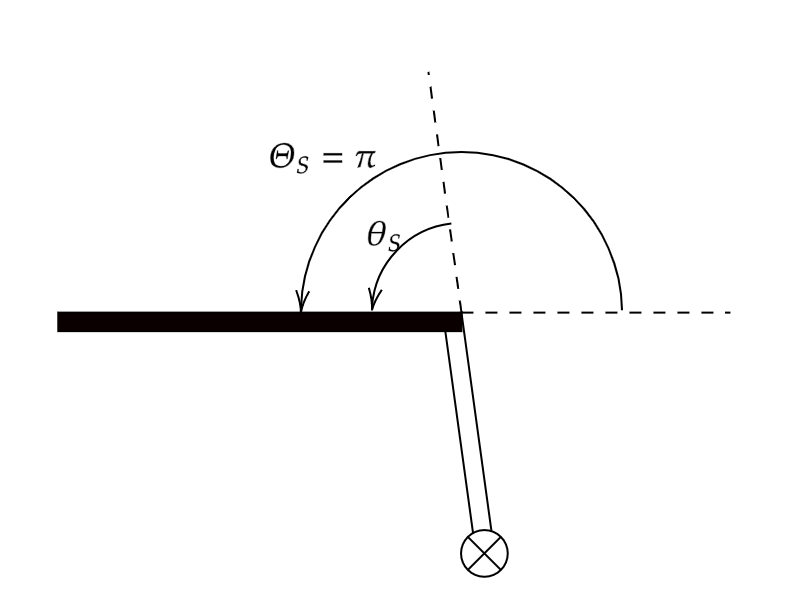
\includegraphics[width=1\textwidth]{PN_horizontal_positive.png}
        \subcaption{$a_{arm}$が正のケース}
        \label{PN_horizontal_positive.png}
      \end{minipage} &
      \begin{minipage}[t]{0.45\textwidth}
        \centering
        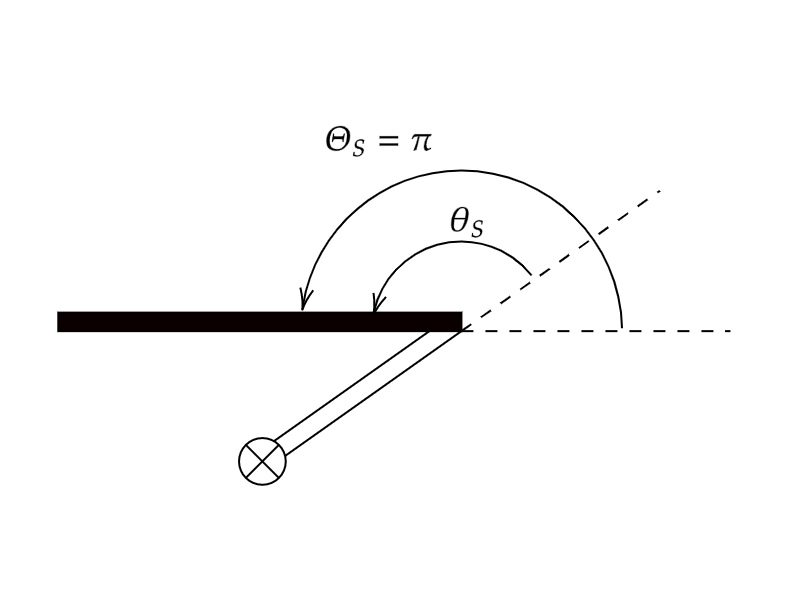
\includegraphics[width=1\textwidth]{PN_horizontal_negative.png}
        \subcaption{$a_{arm}$が負のケース}
        \label{PN_horizontal_negative.png}
      \end{minipage}
    \end{tabular}
    \caption{胴体が水平のとき}
  \end{figure}
\end{enumerate}

\subsection{胴体と上肢の位置関係と角運動量}
式\ref{eq:PB:L_start}~\ref{eq:PB:IG_start}から
$F_S$を決定する。
式\ref{eq:PB:I_start},\ref{eq:PB:IG_start}により
\begin{align}
  & \frac{I}{I_G}F_S\sin\theta_S \cdot L = -Mg\cos\Theta_S \cdot L - Ma_{arm}\cos\theta_S \cdot L
  \\
  & \left( \because L > 0 \right)
  \\
  \Leftrightarrow
  & 0= -Mg\cos\Theta_S - Ma_{arm}\cos\theta_S - \frac{I}{I_G}F_S\sin\theta_S
  \label{eq:PB:FS_end}
\end{align}
式\ref{eq:PB:L_start},\ref{eq:PB:FS_end}を変形して
\begin{align}
  ML\omega^2 \cos\theta_S &= Mg\sin\Theta_S\cos\theta_S &+& Ma\sin\theta_S\cos\theta_S &- &F_S\cos^2\theta_S
  \\
  0 &= -Mg\cos\Theta_S \sin\theta_S 
  &-& Ma_{arm}\cos\theta_S \sin\theta_S 
  &- &\frac{I}{I_G}F_S\sin\theta_S \sin\theta_S
\end{align}
この2式により
\begin{align}
  ML\omega^2 \cos\theta_S 
  &= Mg\left( \sin\Theta_S \cos\theta_S - \cos\Theta_S \sin\theta_S\right)
  - F_S\left( \cos^2\theta_S + \frac{I}{I_G}\sin^2\theta_S \right)
\end{align}
\begin{align}
  \therefore
  F_S\left( \cos^2\theta_S + \frac{I}{I_G}\sin^2\theta_S \right)
  &= -ML\omega^2 \cos\theta_S + Mg \sin(\underbrace{\Theta_S - \theta_S}_{=\theta_W+\frac{1}{2}\pi})
  \label{eq:PB:FS_end}
\end{align}
が分かる。

$F_S$の正負は
式\ref{eq:PB:FS_end}からは簡単に推定されない。
なぜなら、
データ的に$F_S$は大体正なのだが(*要データ確認)、
どちらかの方が十分に大きいという近似は、
正であることを保証しない。
大体正であるためには、
$-ML\omega^2\cos\theta_S < 0$であるうちは
$Mg\sin(\theta_W + \frac{1}{2}\pi) ( > 0 \because -\frac{1}{2}\pi < \theta_W < \frac{1}{2}\pi )$
が大きい必要がある。

ここから先は
$F_S$は大体正であることを前提とする。(だから間違っている可能性がある)

式\ref{eq:PB:IG_start}
\begin{align}
  I_G\dot\omega = F_S \sin\theta_S \cdot L
\end{align}
により、
正の$F_S$は$0 < \theta_S < \pi$であるうちは
角運動量を増加する。
逆に、正の$F_S$は$\pi < \theta_S < 2\pi$のときは
角運動量を減少させる。
つまり、上肢と胴体の角度が重なるときを境に、
正の$F_S$による角運動量の増減は入れ替わる。
より長い間$0 < \theta_S < \pi$、
つまり胴体が上肢より左側にある状態を保ったほうが
角運動量は増加する。

\subsection{胴体と上肢の位置関係と鉛直反力}
肩関節で胴体に対して鉛直方向に働く力の大きさは
\begin{align}
  F_s\sin(\theta_W + \frac{1}{2}\pi)
\end{align}
である。
上肢がより鉛直の時ほど、ある$F_S$に対しては大きな鉛直反力が発生することになる。

だから鉛直反力を大きくして滞空時間を大きくするには
上肢を鉛直に保つことが必要になる。
大抵平行棒の支持スイングにおいては
上肢の角度は鉛直をまたぐ。
逆にまたがないような動作はパフォーマンスが高くない(*要データ確認)。
前半は上肢が鉛直より右側にあり、胴体は上肢より左側にあることが多く、
そして後半は上肢が鉛直より左側にあり、胴体は上肢より右側にあることが多い。
胴体が上肢より左側にある時は上肢が正の方向に加速し、
胴体が上肢より右側にある時は上肢が負の方向に加速することはすでに述べた。
これにより、
胴体が上肢との位置関係を入れ替えるタイミングが
上肢の左右への傾きへ大きな影響を及ぼすことが予想され、
その中でもより上肢を鉛直に保つような動作がパフォーマンスが高くなることが予想される。

\subsection{胴体と上肢の位置関係と回転数}
これまでの議論により
\begin{enumerate}
  \item 胴体と上肢の位置関係により角運動量の増減が決まる
  
  胴体が上肢より左側にある時は角運動量が増加し、
  胴体が上肢より右側にある時は角運動量が減少する。
  \item 胴体と上肢の位置関係により上肢の角度が決まり、鉛直反力が決まる
  
  胴体が上肢より左側にある時は上肢は左に傾き、
  胴体が上肢より右側にある時は上肢は右に傾く。
  上肢がより鉛直に保たれるほど鉛直反力が大きくなる。
\end{enumerate}
ことが分かった。
このことから、
\begin{itemize}
  \item 胴体が上肢より左側にある状況を保ったほうが角運動量は大きくなりやすいが、
  上肢が左に傾きすぎて鉛直反力が小さくなってしまう可能性がある。
\end{itemize}
と考えられる。
そして
「どれほど胴体が上肢より左側にある状況を保ったのか」の指標として
「胴体と上肢が重なるときの上肢の角度」が適していることが
シミュレーションから分かっている。

\begin{figure}[h]
  \begin{tabular}{cc}
    \begin{minipage}[t]{0.45\textwidth}
      \centering
      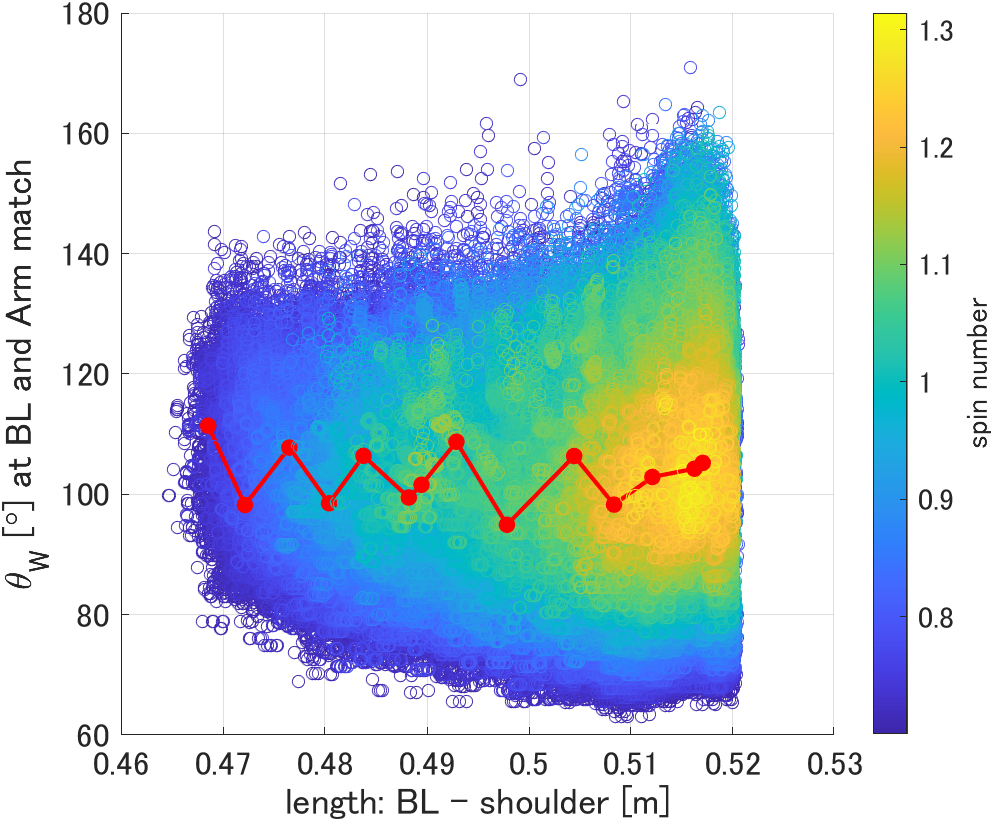
\includegraphics[width=1\textwidth]{PBmodel_theta_at_match.png}
      \subcaption{平行棒モデル: vs 振り子としての長さ}
      \label{PBmodel_theta_at_match.png}
    \end{minipage} &
    \begin{minipage}[t]{0.45\textwidth}
      \centering
      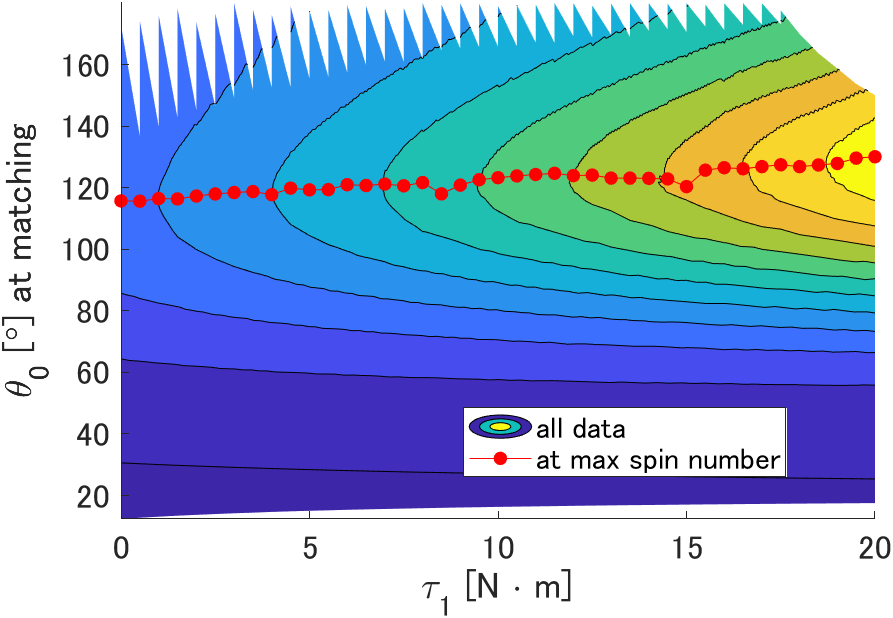
\includegraphics[width=1\textwidth]{1seg_circle_model_theta_at_match.png}
      \subcaption{振り子+剛体単振り子モデル: vs 肩関節にかけるトルクの大きさ}
      \label{1seg_circle_model_theta_at_match.png}
    \end{minipage}
  \end{tabular}
  \caption{回転数と「胴体と上肢が重なるときの上肢の角度」の関係}
\end{figure}



\clearpage
\section{Appendix}
\label{sec:appendix}
\subsection{剛体単振り子の運動方程式}
今回、向心力を考える必要があるから、
剛体単振り子について運動方程式を詳しく考える。

このサブセクションの目的は
図\ref*{Appendix_base_config.png}
の運動方程式が
\begin{align}
  \begin{cases}
    ML\omega^2  &= F_L - \sum_i F_i^L
    \\
    I\dot\omega &= \sum_i F_i^\theta l_i
    \\
    I_G\dot\omega &= -F_\theta L + \sum_i F_i^\theta ( l_i - L )
  \end{cases}
\end{align}
で表されることを確認することである。
重力が外力として存在するような場合、
\begin{align}
  \begin{cases}
    ML\omega^2  &= F_L - \sum_i ( -mg\sin\theta + F_i^L ) = F_L + Mg\sin\theta - \sum_i F_i^L
    \\
    I\dot\omega &= \sum_i ( -mg\cos\theta + F_i^\theta ) l_i = -MgL\cos\theta + \sum_i F_i^\theta l_i
    \\
    I_G\dot\omega &= -F_\theta L + \sum_i F_i^\theta ( l_i - L )
  \end{cases}
\end{align}
となる。


\begin{figure}[h]
  \centering
  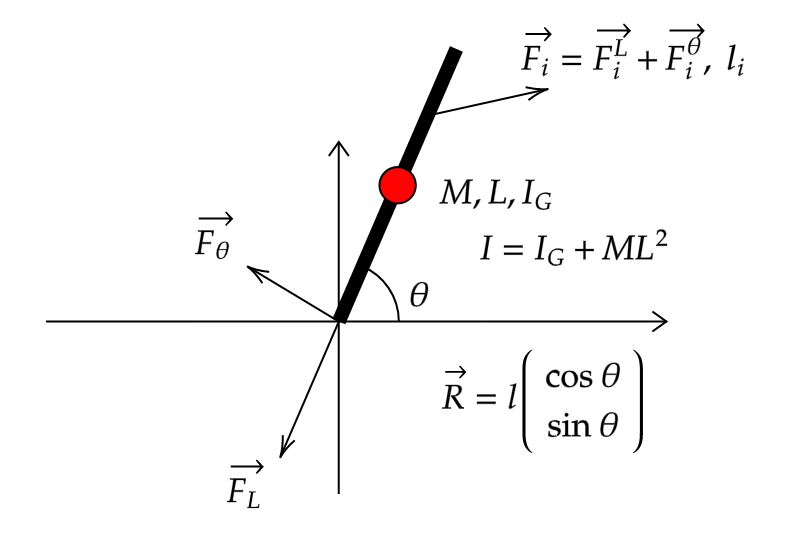
\includegraphics[width = 0.6\textwidth]{Appendix_base_config.png}
  \caption{剛体振り子の基本設定}
  \label{Appendix_base_config.png}
\end{figure}

まず初めに、
ラグランジュ運動方程式によって
簡単に運動方程式を導出する。
しかしラグランジュ方程式から
物理的解釈、理解をすることが難しいので、
のちにニュートン力学からも運動方程式を導出する。

\subsubsection{ラグランジアンによる導出}

ラグランジアンから式を導出するには、
導出したい文字式を一度時間変化するとして計算し、
最後に時間変化しない、という条件を代入する必要がある。
そこで回転軸及び剛体の重心が自由に動くように、
$L=L(t)$、$x_\theta=x_\theta(t)$であるような状況
(図\ref{Appendix_lag_config.png})を考える。

\begin{figure}[h]
  \centering
  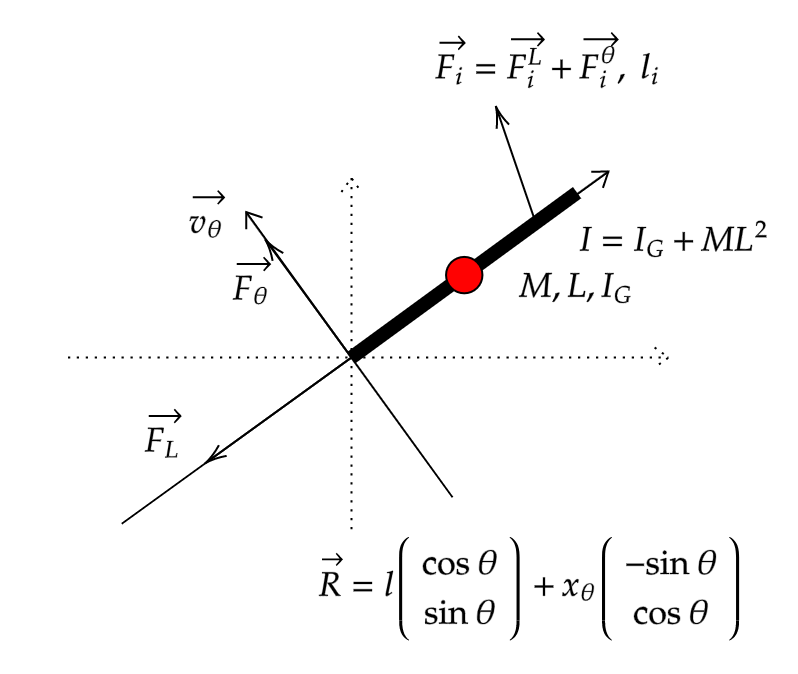
\includegraphics[width = 0.6\textwidth]{Appendix_lag_config.png}
  \caption{ラグランジアンの際の設定}
  \label{Appendix_lag_config.png}
\end{figure}

重心速度$\vec{V}$は
\begin{align}
  \vec{V} &= 
  \dot{L}
  \begin{pmatrix}
    \cos\theta
    \\
    \sin\theta
  \end{pmatrix}
  + L\omega
  \begin{pmatrix}
    -\sin\theta
    \\
    \cos\theta
  \end{pmatrix}
  + v_\theta \begin{pmatrix}
    -\sin\theta
    \\
    \cos\theta
  \end{pmatrix}
  + x_\theta \omega \begin{pmatrix}
    -\cos\theta
    \\
    -\sin\theta
  \end{pmatrix}
  \\
  &= 
  ( \dot{L} - x_\theta \omega )
  \begin{pmatrix}
    \cos\theta
    \\
    \sin\theta
  \end{pmatrix}
  + ( L\omega + v_\theta )
  \begin{pmatrix}
    -\sin\theta
    \\
    \cos\theta
  \end{pmatrix}
\end{align}


力学的エネルギー$T$は
剛体の質量$M$、重心周りの慣性モーメント$I_G$、角度$\theta$、重心までの距離$L$を用いて
\begin{align}
  T = 
  \frac{1}{2}I_G\omega^2
  + \frac{1}{2}M
  \Bigl[ (\dot{L} - x_\theta \omega)^2 + (L\omega + v_\theta)^2 \Bigr]
\end{align}
で表される。
位置エネルギー$U$は
\begin{align}
  U = Mg ( L\sin\theta + x_\theta \cos\theta )
\end{align}
で表される。
これによってラグランジアン$Lag$は
\begin{align}
  Lag &=
  T - U
  \\
  &= 
  \frac{1}{2}I_G\omega^2
  + \frac{1}{2}M
  \Bigl[ (\dot{L} - x_\theta \omega)^2 + (L\omega + v_\theta)^2 \Bigr]
  - Mg ( L\sin\theta + x_\theta \cos\theta )
\end{align}
と表される。

\subsubsection*{回転の運動方程式}
ラグランジュ方程式は
\begin{align}
  \frac{d}{dt}\frac{\partial Lag}{\partial \omega} - \frac{\partial Lag}{\partial \theta} = Q_\theta
  \label{eq:lag:theta_start}
\end{align}
と表現される。
ただし$Q_\theta$は回転に関する一般化力で、トルクに相当し、
\begin{align}
  Q_\theta = \sum_i F_i^\theta l_i
\end{align}
が成り立つ。
また、ラグランジュ方程式の各項が
\begin{align}
  \frac{d}{dt}\frac{\partial Lag}{\partial \omega}
  &= \frac{d}{dt}\frac{\partial }{\partial \omega}
  \left(
    \frac{1}{2}I_G\omega^2
    + \frac{1}{2}M
    \Bigl[ (\dot{L} - x_\theta \omega)^2 + (L\omega + v_\theta)^2 \Bigr]
    - Mg ( L\sin\theta + x_\theta \cos\theta )
  \right)
  \\
  &= \frac{d}{dt} \left( I_G\omega + \frac{1}{2}ML\cdot 2(L\omega + v_\theta) \right)
  \\
  & \ \ \ \ \left( \because x_\theta = 0 \right)
  \\
  &= I_G\dot\omega + ML^2\dot\omega
  \\
  &= (I_G + ML^2)\dot\omega
\end{align}
\begin{align}
  \frac{\partial Lag}{\partial \theta}
  &= \frac{\partial }{\partial \theta}
  \left(
    \frac{1}{2}I_G\omega^2
    + \frac{1}{2}M
    \Bigl[ (\dot{L} - x_\theta \omega)^2 + (L\omega + v_\theta)^2 \Bigr]
    - Mg ( L\sin\theta + x_\theta \cos\theta )
  \right)
  \\
  &= \frac{\partial }{\partial \theta}\left( - Mg ( L\sin\theta + x_\theta \cos\theta ) \right)
  \\
  & \ \ \ \ \left( \because x_\theta = 0 \right)
  \\
  &= -MgL\cos\theta
\end{align}
のように計算される。
よって式\ref{eq:lag:theta_start}は
\begin{align}
  & (ML^2 + I_G)\dot\omega - ( -MgL\cos\theta ) = \sum_i F_i^\theta l_i
  \\
  \Leftrightarrow
  & (ML^2 + I_G)\dot\omega = -MgL\cos\theta + \sum_i F_i^\theta l_i
  \\
  \Leftrightarrow
  & I\dot\omega = -MgL\cos\theta + \sum_i F_i^\theta l_i
  \label{eq:lag:theta_end}
\end{align}
実はラグランジュ方程式に一般化力を加えるときは正負が不安なのだが、
式\ref{eq:lag:theta_end}の重力の作用を見て
合っていることの確認もとれた。

\subsubsection*{動径方向の運動方程式}
ラグランジュ方程式は
\begin{align}
  \frac{d}{dt}\frac{\partial Lag}{\partial \dot{L}} - \frac{\partial Lag}{\partial L} = Q_L
  \label{eq:lag:length_start}
\end{align}
と表現される。
ただし$Q_L$は動径方向に関する一般化力で、原点が広がる力を正にとったものに相当し、
\begin{align}
  Q_L = -F_L +  \sum_i F_i^L
\end{align}
が成り立つ。
また、ラグランジュ方程式の各項が
\begin{align}
  \frac{d}{dt}\frac{\partial Lag}{\partial \dot{L}}
  &= \frac{d}{dt}\frac{\partial }{\partial \dot{L}}
  \left(
    \frac{1}{2}I_G\omega^2
    + \frac{1}{2}M
    \Bigl[ (\dot{L} - x_\theta \omega)^2 + (L\omega + v_\theta)^2 \Bigr]
    - Mg ( L\sin\theta + x_\theta \cos\theta )
  \right)
  \\
  & = \frac{d}{dt}\left( \frac{1}{2}M \cdot 2(\dot{L} - x_\theta \omega)\right)
  \\
  &= M( \ddot{L} - v_\theta \omega - x_\theta \dot\omega )
  \\
  & \ \ \ \ \left( \because x_\theta = 0 \right)
  \\
  &= M \ddot{L}
\end{align}
\begin{align}
  \frac{\partial Lag}{\partial L}
  &= \frac{\partial }{\partial L}
  \left(
    \frac{1}{2}I_G\omega^2
    + \frac{1}{2}M
    \Bigl[ (\dot{L} - x_\theta \omega)^2 + (L\omega + v_\theta)^2 \Bigr]
    - Mg ( L\sin\theta + x_\theta \cos\theta )
  \right)
  \\
  &= \frac{1}{2}M \cdot 2\omega(L\omega + v_\theta) - Mg\sin\theta
  \\
  & \ \ \ \ \left( \because x_\theta = 0 \right)
  \\
  &= ML\omega^2 - Mg\sin\theta
\end{align}
のように計算される。
よって式\ref{eq:lag:length_start}は
\begin{align}
  M\ddot{L} - ( ML\omega^2 - MgL\sin\theta ) = -F_L + \sum_i F_i^L
\end{align}
となる。
ここで剛体という条件から$\ddot{L} = 0$を代入すると
\begin{align}
  & 0 - ( ML\omega^2 - MgL\sin\theta ) = -F_L + \sum_i F_i^L
  \\
  \Leftrightarrow
  & ML\omega^2 = F_L + MgL\sin\theta - \sum_i F_i^L
  \label{eq:lag:length_end}
\end{align}
と求められる。
重力による項$-MgL\sin\theta$は各質点にかかる重力$\vec{f}_g$の
動径方向成分の総和であるので、
$\sum_i F_i^L$に吸収してもよい。

\subsubsection*{回転方向の並進運動方程式}
ラグランジュ方程式は
\begin{align}
  \frac{d}{dt}\frac{\partial Lag}{\partial v_\theta} - \frac{\partial Lag}{\partial x_\theta} = Q_{F_\theta}
  \label{eq:lag:Ftheta_start}
\end{align}
と表現される。
ただし$Q_L$は回転方向に関する一般化力で、その時点での回転方向への力に相当し、
\begin{align}
  Q_{F_\theta} = F_\theta + \sum_i F_i^\theta
\end{align}
が成り立つ。
また、ラグランジュ方程式の各項が
\begin{align}
  \frac{d}{dt}\frac{\partial Lag}{\partial v_\theta}
  &= \frac{d}{dt}\frac{\partial }{\partial v_\theta}
  \left(
    \frac{1}{2}I_G\omega^2
    + \frac{1}{2}M
    \Bigl[ (\dot{L} - x_\theta \omega)^2 + (L\omega + v_\theta)^2 \Bigr]
    - Mg ( L\sin\theta + x_\theta \cos\theta )
  \right)
  \\
  & = \frac{d}{dt}\left( \frac{1}{2}M \cdot 2(L\omega + v_\theta )\right)
  \\
  &= M( \dot{L}\omega + L\dot\omega + a_\theta )
  \\
  & \ \ \ \ \left( \because x_\theta = 0, L = const. \right)
  \\
  &= M L \dot\omega
\end{align}
\begin{align}
  \frac{\partial Lag}{\partial x_\theta}
  &= \frac{\partial }{\partial x_\theta}
  \left(
    \frac{1}{2}I_G\omega^2
    + \frac{1}{2}M
    \Bigl[ (\dot{L} - x_\theta \omega)^2 + (L\omega + v_\theta)^2 \Bigr]
    - Mg ( L\sin\theta + x_\theta \cos\theta )
  \right)
  \\
  &= 0 - Mg\cos\theta
  \\
  &= - Mg\cos\theta
\end{align}
のように計算される。
よって式\ref{eq:lag:length_start}は
\begin{align}
  & M L \dot\omega - ( - Mg\cos\theta ) = F_\theta + \sum_i F_i^\theta
  \\
  \Leftrightarrow
  & M L \dot\omega = - Mg \cos\theta + F_\theta + \sum_i F_i^\theta
  \\
  \Rightarrow
  & M L^2 \dot\omega = - Mg L \cos\theta + F_\theta L + \sum_i F_i^\theta L
  \label{eq:lag:x_middle}
\end{align}
となる。
ここで式\ref{eq:lag:theta_end}を変形する。
\begin{align}
  I\dot\omega 
  &= -MgL\cos\theta + \sum_i F_i^\theta l_i
  \\
  &= -MgL\cos\theta + \sum_i F_i^\theta (l_1 - L) + \sum_i F_i^\theta L
  \\
  \Leftrightarrow
  \sum_i F_i^\theta L
  &= I\dot\omega + MgL\cos\theta - \sum_i F_i^\theta (l_1 - L)
\end{align}
よって式\ref{eq:lag:x_middle}は
\begin{align}
  & M L^2 \dot\omega = - Mg L \cos\theta + F_\theta L + \sum_i F_i^\theta L
  \\
  \Leftrightarrow
  & M L^2 \dot\omega = - Mg L \cos\theta + F_\theta L + I\dot\omega + MgL\cos\theta - \sum_i F_i^\theta (l_1 - L)
  \\
  \Leftrightarrow
  & ( M L^2 - I ) \dot\omega = F_\theta L - \sum_i F_i^\theta (l_1 - L)
  \\
  \Leftrightarrow
  & -I_G \dot\omega = F_\theta L - \sum_i F_i^\theta (l_1 - L)
  \\
  \Leftrightarrow
  & I_G \dot\omega = - F_\theta L + \sum_i F_i^\theta (l_1 - L)
  \label{eq:lag:Ftheta_end}
\end{align}
と変形され、$F_\theta$に関する方程式を得た。

よってまとめると、
式\ref{eq:lag:theta_end}, \ref{eq:lag:length_end}, \ref{eq:lag:Ftheta_end}より
\begin{align}
  \begin{cases}
    ML\omega^2 &= F_L + MgL\sin\theta - \sum_i F_i^L
    \\
    I\dot\omega &= -MgL\cos\theta + \sum_i F_i^\theta l_i
    \\
    I_G\dot\omega &= -F_\theta L + \sum_i F_i^\theta ( l_i - L )
  \end{cases}.
\end{align}

\clearpage
\subsubsection{ニュートン力学での導出}
\label{subsubsec:newton}

回転軸からの距離$l$に対して質量密度を$m=m(l)$で与える。
この時
\begin{align}
  \int m dl = M, \ \ \ \ \ \
  \frac{\int ml dl}{\int m dl} = L, \ \ \ \ \ \
  \int ml^2 dl = I
\end{align}
である。
回転軸からの距離$l$にある質量$m$に関して、
動径方向の力を$f_l=f_l(l)$、
回転方向の力を$f_\theta=f_\theta(l)$
として運動方程式を考えると
\begin{align}
  \begin{cases}
    f_l = -ml\omega^2
    \\
    f_\theta = ml\dot\omega
  \end{cases}
\end{align}
となる。

動径方向の力に関して回転軸からの距離$l$で積分すると
\begin{align}
  \int f_l dl 
  &= \int -ml\omega^2 dl
  \\
  &= -\omega^2 \int ml dl
  \\
  &= -\omega^2 \int m dl \cdot \frac{ \int ml dl }{\int m dl }
  \\
  &= -\omega^2 M \cdot L
  \\
  &= -ML\omega^2
\end{align}
が分かる。
微小質点にかかる剛体方向の力を積分した左辺が
外力の合計に等しいことから、
\begin{align}
  \int f_l dl = -F_L + \sum_i F_i^{L}
\end{align}
を考えるのは自然であろう。
よって動径方向の運動方程式は
\begin{align}
  & -F_L + \sum_i F_i^{L} = -ML\omega^2
  \\
  \Leftrightarrow
  & ML\omega^2 = F_L - \sum_i F_i^{L}
  \label{eq:newton:length_end}
\end{align}
となり、ラグランジアンからの導出結果と一致する。

回転方向は少しややこしい。
まず、回転方向の力$f_\theta$を
剛体の内力$f_\theta^{in}$と外力$f_\theta^{out}$に分類する。
つまり回転方向の運動方程式は
\begin{align}
  f_\theta^{in} + f_\theta^{out} = ml\dot\omega
  \label{eq:newton:theta_start}
\end{align}
と表される。
正直これから書く内容は定かではない。

回転軸周りの慣性モーメント$I$を式中に登場させるために、
\ref{eq:newton:theta_start}の両辺に回転軸からの距離$l$をかけて、積分する。
\begin{align}
  \int f_\theta^{in} l dl + \int f_\theta^{out} l dl
  &= \int ml^2\dot\omega dl
  \\
  &= \dot\omega\int ml^2 dl
  \\
  &= \dot\omega I = I\dot\omega
\end{align}

ここで、内力が角運動量を変化させないことから(この部分が特に定かではない)
\begin{align}
  \int f_\theta^{in} l dl = 0
\end{align}
となる。
これは、そのような$f_\theta^{in}$が発生すると考えたほうが分かりやすい。
この式から
\begin{align}
  f_\theta^{in} = 0
\end{align}
を導くことは数学的に間違っていることは簡単に分かり、
そして物理的な解釈からも否定される。
というのも、片端が固定された棒の反対の端を指で動かす場合を考える。
指からの力、つまり外力が働く部分は端のみであるが、
もちろん外力のかからない真ん中の部分も押された回転方向に動く。
つまり、その向きに内力が発生していることになる。
よって内力による合計のトルクは0であるが、
回転方向の内力がいたるところで0であるわけではない。

次に外力について考える。
筆者はこの外力について考えるとき、
外力による合計のトルクに関して
外力の回転方向成分を合計した力$F_\theta^G$に対して
\begin{align}
  \int f_\theta^{out} l dl = F_\theta^G L
\end{align}
であるはずという観念があり、
大変苦労した。
これは簡単に否定されるので、
先に否定しておく。
質量$m_0$である質点を、回転軸から$l_1, l_2$の部分に置く。
それぞれの質点に回転方向への成分が$F_1, F_2$である外力を作用させる。
回転軸周りの合計トルクは
\begin{align}
  F_1 l_1 + F_2 l_2
  \neq
  (F_1 + F_2) \frac{l_1 + l_2}{2}
\end{align}
である。
これによって
\begin{align}
  \int f_\theta^{out} l dl \neq F_\theta^G L
\end{align}
が証明された。

しかし、
\begin{align}
  \int f_\theta^{out} l dl = F_\theta^G L
\end{align}
が成り立つような外力が存在する。
それは質量に比例する力である。
重力や慣性力がその例となる。
厳密には各質点に同じ大きさでかかる力も満たすが、
今回は考えない。
比例定数を$A_f$とすると、
\begin{align}
  \int f_\theta^{out} l dl
  &= \int A_f m l dl
  \\
  &= A_f \int m l dl
  \\
  &= A_f \int m dl \frac{\int mldl}{\int mdl}
  \\
  &= A_f M L
\end{align}
また、外力の回転方向成分の合計である$F_\theta^G$は
\begin{align}
  F_\theta^G
  = \int f_\theta^{out} dl
  = \int A_f m dl
  = A_f \int mdl
  = A_f M
\end{align}
であるから、
\begin{align}
  \int f_\theta^{out} l dl = F_\theta^G L
\end{align}
が成り立つ。
よって回転方向の運動方程式は
\begin{align}
  I\dot\omega 
  &= \int f_\theta^{out} l dl
  \\
  & \ \ \left( \mathrm{特に各質点に質量に比例してかかる力だけの場合は} \right)
  \\
  &= F_\theta^G L
\end{align}
となる。
重力や添え字$i$で関連付けられた外力を具体的に考慮すると、
\begin{align}
  & f_\theta^{out}(l) = -m(l)g \cos\theta + F_\theta \delta(l) + \sum_i F_i^\theta \delta( l - l_i )
  \label{eq:newton:f_theta_out_conf}
  \\
  \Rightarrow
  & \int f_\theta^{out} l dl = -MgL \cos\theta + \sum_i F_i^\theta l_i
\end{align}
であるから、
\begin{align}
  I\dot\omega 
  = \int f_\theta^{out} l dl
  = -MgL\cos\theta + \sum_i F_i^\theta l_i
  \label{eq:newton:theta_end}
\end{align}
が分かり、
ラグランジアンからの導出結果と一致する。

最後に、$F_\theta$に関する運動方程式を導出する。
式\ref{eq:newton:theta_end}から
\begin{align}
  I\dot\omega 
  &= \int_0^\infty f_\theta^{out} l dl
  \\
  &= \int_0^\infty f_\theta^{out} ( l - L ) dl
  + \int_0^\infty f_\theta^{out} L dl
  \\
  &= \int_0^\infty f_\theta^{out} ( l - L ) dl
  + L \int_0^\infty f_\theta^{out} dl
  \\
  &= \int_0^\infty f_\theta^{out} ( l - L ) dl
  + L \cdot ( ML\dot\omega) 
\end{align}
具体的に式\ref{eq:newton:f_theta_out_conf}により重力と外力を考慮すると
\begin{align}
  I\dot\omega
  &= \int_0^\infty f_\theta^{out} ( l - L ) dl
  + L \cdot ( ML\dot\omega) 
  \\
  &= Mg(L - L) \cos\theta + F_\theta ( 0 - L ) + \sum_i F_i^\theta ( l_1 - L ) + ML^2\dot\omega
  \\
  & \Leftrightarrow
  ( I - ML^2 ) \dot\omega = - F_\theta L + \sum_i F_i^\theta ( l_1 - L )
  \\
  & \Leftrightarrow
  I_G \dot\omega = - F_\theta L + \sum_i F_i^\theta ( l_1 - L )
  \label{eq:newton:Ftheta_end}
\end{align}

よってまとめると、
式\ref{eq:newton:length_end},\ref{eq:newton:theta_end},\ref{eq:newton:Ftheta_end}
により
\begin{align}
  \begin{cases}
    ML\omega^2 &= F_L - \sum_i F_i^{L}
    \\
    I\dot\omega &= -MgL\cos\theta + \sum_i F_i^\theta l_i
    \\
    I_G \dot\omega &= - F_\theta L + \sum_i F_i^\theta ( l_1 - L )
  \end{cases}
\end{align}


\end{document}